\section{Evaluation}
\label{sec:evaluation}

To evaluate our framework, we developed a prototype for a Smart Home application
that combines together Intel \ac{SGX}, ARM TrustZone and Sancus. In this
chapter, we  introduce our Smart Home environment and motivate security
requirements (\cref{eval:intro}); then, we describe the hardware and software
setup of our evaluation (\cref{eval:test-env}). After that, we provide a
detailed performance analysis of our application (\cref{eval:microb}), and
finally discuss \ac{TCB} size and development effort (\cref{eval:macrob}).

\subsection{Smart Homes}
\label{eval:intro}

A smart home is a residential property integrated with technology to remotely
control appliances and systems, such as lighting, heating and cooling, and
entertainment. The adoption of smart home devices has increased rapidly, with an
estimated 250 million smart homes worldwide in 2021, expected to reach 350
million by
2023\footnote{\url{https://www.statista.com/topics/2430/smart-homes}}. Despite
the benefits such as enhanced comfort and energy efficiency, security concerns
arise from inadequate security measures in many smart home devices. Studies like
\cite{davis2020vulnerability} have shown that many vulnerabilities come from
poor authentication, missing encryption, insecure software updates, and
insufficient access control, leading to potential privacy violations and
unauthorized access to personal information and control of home devices.

Thus, our framework can be utilized in the context of smart homes to provide
robust security guarantees. Through the use of \acp{TEE}, both code and data are
protected in use, and attestation ensures code integrity. Additionally, our
deployment approach supports secure software updates and guarantees that all
connections are encrypted and mutually authenticated. This eliminates a broad
range of attacks while minimizing the development and deployment effort.

\subsection{Testing environment}
\label{eval:test-env}

\begin{figure}[t]
  \hspace*{-0.3cm}
  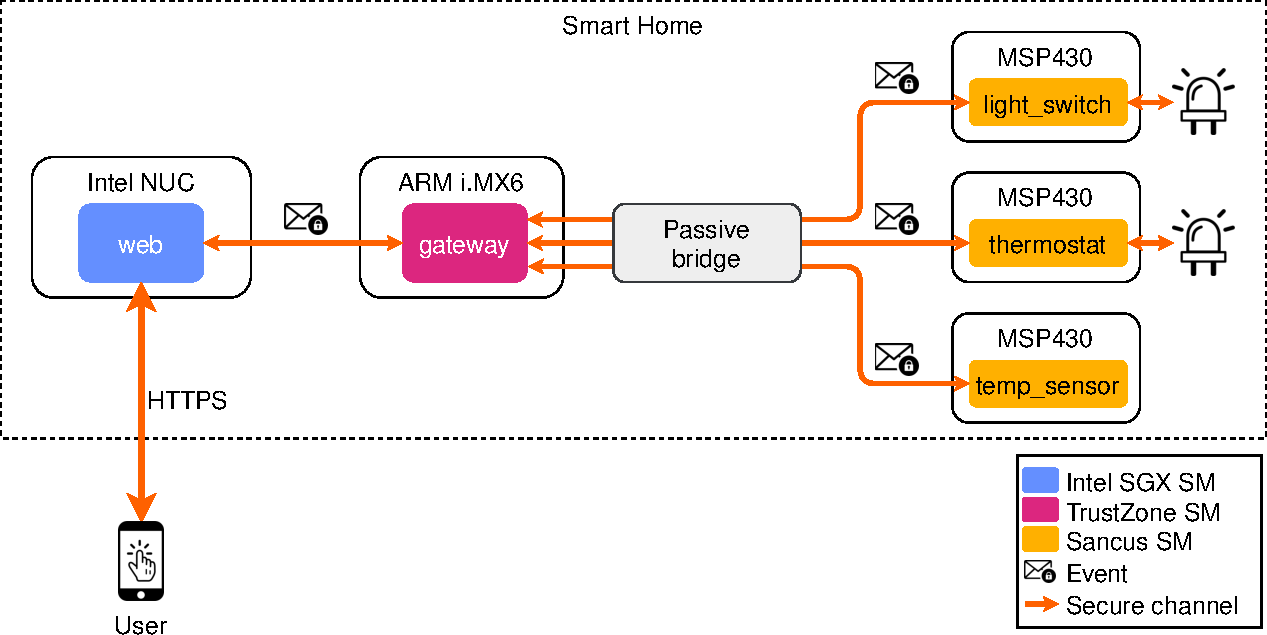
\includegraphics[width=0.7\columnwidth]{graphics/smart-home.drawio.pdf}

  \caption{Setup of our \emph{smart home} application. Each \ac{SM} is deployed
  on a different node, either running Intel \ac{SGX}, TrustZone or Sancus. All
  communication between modules is encrypted and authenticated by our framework,
  while the communication between \web{} and users relies on HTTPS and mutually
  authenticated. Sancus nodes are connected via UART to a passive bridge, which
  converts between UART streams and TCP/IP.}
  \label{fig:eval-setup}
\end{figure}

To evaluate our framework, we developed a prototype for a small smart home
application consisting of three simulated IoT devices: a temperature sensor, a
smart thermostat and a light switch. A smart home gateway, similar to existing
projects such as Home Assistant\footnote{\url{https://www.home-assistant.io/}},
manages the IoT devices and enforces some custom-defined logic, e.g., to
automatically turn on or off the heating if the temperature goes below or above
predefined thresholds. Furthermore, a web application is made available to local
and remote users, to monitor the house and perform some operations on demand,
e.g., to switch the lights on or off. Both smart thermostat and light switch are
connected via Secure I/O to an LED, indicating whether heating and lights are on
or off at a certain time. The source code of our prototype is publicly available
on
Github\footnote{\url{https://github.com/AuthenticExecution/examples/tree/main/smart-home}}.

We implemented an application such as described above using five \acp{SM}:
\begin{itemize}
  \item \web: Exposes a web application to allow external users to interact with
  the smart home;
  \item \gateway: Manages all the IoT devices and enforces a user-defined logic,
  while at the same time interacting with \web{} to send status data and receive
  commands from external users;
  \item \tempsensor: Simulates a sensor that provides the current temperature in
  the house;
  \item \thermostat: Simulates a smart thermostat, to enable or disable the
  heating system;
  \item \light: Simulates a smart light switch, to enable or disable the lights.
\end{itemize}

As depicted in \cref{fig:eval-setup}, we deployed our smart home application as
follows:
%
\begin{itemize}
  \item \web{} as an Intel \ac{SGX} \ac{SM}, on an Intel NUC7i3BNHXF with Intel
  Core i3-7100U;
  \item \gateway{} as a TrustZone \ac{SM}, on a BD-SL-i.MX6 board with ARM
  Cortex-A9 running at 1GHz;
  \item \tempsensor, \thermostat{} and \light{} as Sancus \acp{SM}, on three
  different 16-bit OpenMSP430 microcontrollers running at 8MHz.
\end{itemize}
%
In our setup, all nodes communicate over TCP/IP in the same local network;
However, multiple deployment strategies may be adopted, e.g., deploying \web{}
in a public cloud. Since our Sancus microcontrollers can only communicate
through UART, we wrote a Python script that acts as a passive bridge, converting
UART streams to TCP/IP packets and vice versa without being able to decrypt or
manipulate the content of events. 

All communication is end-to-end protected from the user to the IoT devices. As
shown in the figure, communication between \acp{SM} is carried over encrypted
and authenticated \emph{events}, leveraging our framework (\cref{sec:design}).
Instead, the communication channel between \web{} and the user is encrypted
using HTTPS. User and \web{} mutually authenticate each other: \web{} is
authenticated by the user during the TLS handshake, during which \web{} presents
an ephemeral X.509 certificate generated after successful attestation; the user,
instead, authenticates by providing a \emph{secret token}, similarly to session
cookies or \acp{JWT}.

\subsection{Performance Benchmarks}
\label{eval:microb}

We analyzed the performance of the Smart Home application introduced above.
Cryptographic overhead was assessed per node and an end-to-end evaluation was
conducted by measuring the round-trip time of an event sent from \web{} to
\light{} and return. The impact of a module update was evaluated by measuring
application downtime during the update.

\subsubsection{Cryptographic operations}
\label{eval:microb-crypto}

\begin{figure*}[t]
  \hspace*{-0.3cm}
  \begin{subfigure}{.48\linewidth}
    \centering
    \resizebox{.9\linewidth}{!} {
      % This file was created with tikzplotlib v0.10.1.
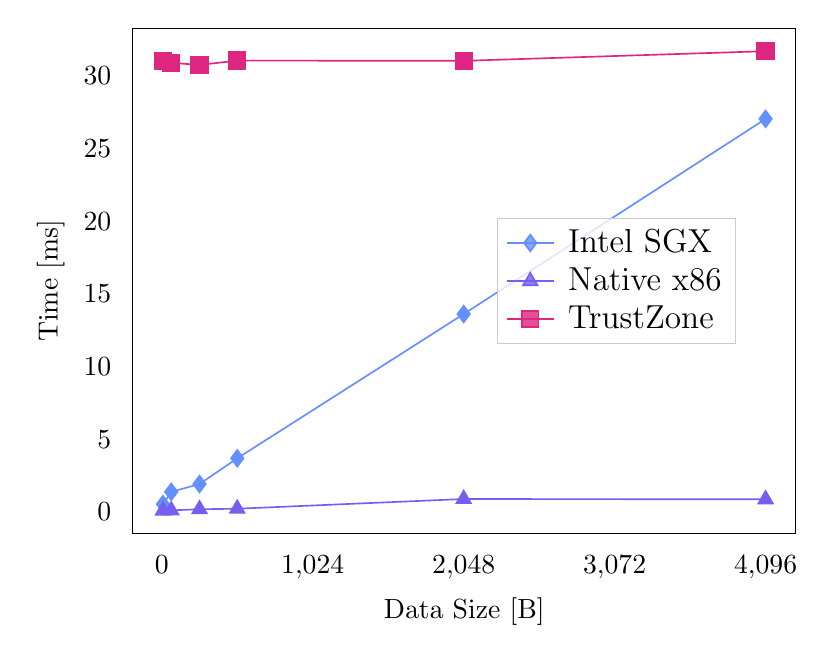
\begin{tikzpicture}

\definecolor{cornflowerblue100143255}{RGB}{100,143,255}
\definecolor{darkgray176}{RGB}{176,176,176}
\definecolor{lightgray204}{RGB}{204,204,204}
\definecolor{mediumslateblue12094240}{RGB}{120,94,240}
\definecolor{mediumvioletred22038127}{RGB}{220,38,127}

\begin{axis}[
scaled y ticks=false,
clip=false,
height=8cm,
legend cell align={left},
legend style={/tikz/every even column/.append style={column sep=0.3cm},/tikz/every odd column/.append style={column sep=0.1cm},font=\large,
  fill opacity=0.8,
  draw opacity=1,
  text opacity=1,
  at={(0.91,0.5)},
  anchor=east,
  draw=lightgray204
},
minor xtick={},
minor ytick={},
tick align=outside,
tick pos=left,
width=10cm,
x grid style={darkgray176},
xlabel={Data Size [B]},
xmin=-196.4, xmax=4300.4,
xtick style={color=black,draw=none},
xtick={0,1024,2048,3072,4096},
y grid style={darkgray176},
ylabel={Time [ms]},
ymin=-1.48298422727273, ymax=33.2882687727273,
ytick style={color=black,draw=none},
ytick={-5,0,5,10,15,20,25,30,35}
]
\addplot [semithick, cornflowerblue100143255, mark=diamond*, mark size=3, mark options={solid}]
table {%
8 0.543356363636385
64 1.38966545454548
256 1.92912000000002
512 3.69842000000002
2048 13.62382
4096 27.0503290909091
};
\addlegendentry{Intel SGX}
\addplot [semithick, mediumslateblue12094240, mark=triangle*, mark size=3, mark options={solid}]
table {%
8 0.0975272727272727
64 0.118718181818182
256 0.194054545454545
512 0.229927272727273
2048 0.898545454545455
4096 0.877809090909091
};
\addlegendentry{Native x86}
\addplot [semithick, mediumvioletred22038127, mark=square*, mark size=3, mark options={solid}]
table {%
8 31.0168481818182
64 30.9077572727273
256 30.7623027272727
512 31.0623027272727
2048 31.0441209090909
4096 31.7077572727273
};
\addlegendentry{TrustZone}
\end{axis}

\end{tikzpicture}

    }
    \caption{\aes-128}
    \label{fig:eval-crypto-aes}
  \end{subfigure}
  \begin{subfigure}{.48\linewidth}
    \centering
    \resizebox{.9\linewidth}{!} {
      % This file was created with tikzplotlib v0.10.1.
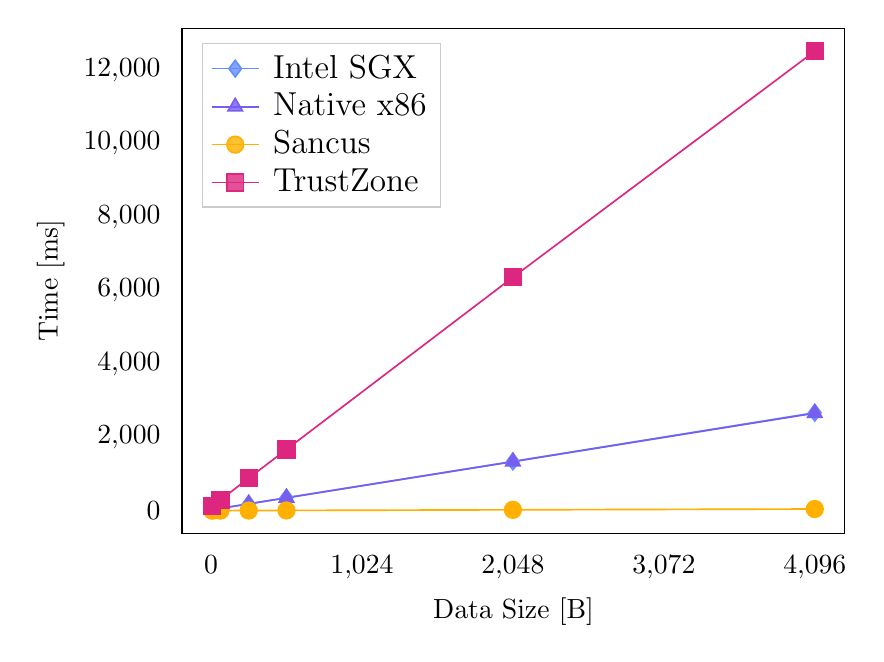
\begin{tikzpicture}

\definecolor{cornflowerblue100143255}{RGB}{100,143,255}
\definecolor{darkgray176}{RGB}{176,176,176}
\definecolor{lightgray204}{RGB}{204,204,204}
\definecolor{mediumslateblue12094240}{RGB}{120,94,240}
\definecolor{mediumvioletred22038127}{RGB}{220,38,127}
\definecolor{orange2551760}{RGB}{255,176,0}

\begin{axis}[
scaled y ticks=false,
clip=false,
height=8cm,
legend cell align={left},
legend style={/tikz/every even column/.append style={column sep=0.3cm},/tikz/every odd column/.append style={column sep=0.1cm},font=\large,
  fill opacity=0.8,
  draw opacity=1,
  text opacity=1,
  at={(0.03,0.97)},
  anchor=north west,
  draw=lightgray204
},
minor xtick={},
minor ytick={},
tick align=outside,
tick pos=left,
width=10cm,
x grid style={darkgray176},
xlabel={Data Size [B]},
xmin=-196.4, xmax=4300.4,
xtick style={color=black,draw=none},
xtick={0,1024,2048,3072,4096},
y grid style={darkgray176},
ylabel={Time [ms]},
ymin=-625.623280477273, ymax=13148.3711400227,
ytick style={color=black,draw=none},
ytick={-2000,0,2000,4000,6000,8000,10000,12000,14000}
]
\addplot [semithick, cornflowerblue100143255, mark=diamond*, mark size=3, mark options={solid}]
table {%
8 24.6539018181818
64 61.0155927272727
256 184.691729090909
512 350.765883636364
2048 1340.85512
4096 2669.05358363636
};
\addlegendentry{Intel SGX}
\addplot [semithick, mediumslateblue12094240, mark=triangle*, mark size=3, mark options={solid}]
table {%
8 25.7767363636364
64 61.7357727272727
256 185.228163636364
512 350.051881818182
2048 1335.13959090909
4096 2656.71204545455
};
\addlegendentry{Native x86}
\addplot [semithick, orange2551760, mark=*, mark size=3, mark options={solid}]
table {%
8 0.467375
64 1.072875
256 3.148875
512 5.916875
2048 22.524875
4096 44.668875
};
\addlegendentry{Sancus}
\addplot [semithick, mediumvioletred22038127, mark=square*, mark size=3, mark options={solid}]
table {%
8 120.816848181818
64 290.907757272727
256 886.598666363636
512 1668.38048454545
2048 6359.67139363636
4096 12522.2804845455
};
\addlegendentry{TrustZone}
\end{axis}

\end{tikzpicture}

    }
    \caption{\spongent-128}
    \label{fig:eval-crypto-spongent}
  \end{subfigure}
  \caption{Average timings to perform encryption using \aes-128 and
  \spongent-128 on different \acp{TEE}. As a reference, we also measured the
  average time spent on a Linux x86 process without \ac{TEE} protection (i.e.,
  the \emph{Native x86} line). All measurements are in milliseconds.}
  \label{fig:eval-crypto}
\end{figure*}

\cref{fig:eval-crypto} shows the average time calculated on each \acp{TEE} to
perform crypto operations using either \aesgcm{} or \spongent{} as authenticated
encryption library, with 128 bits of security. We used different sizes for the
data to encrypt, ranging from 8 to 4096 bytes. To provide a reference, we also
carried out the same experiments on a simple Linux x86 process without \ac{TEE}
protection, running on the Intel \ac{SGX} node, whose results are depicted in
the third column (\emph{Native x86}). The plots show average timings computed
over 110 iterations, except that Sancus values have been extrapolated from
previous experiments~\cite{noorman_sancus2}.

Modern x86 and ARM processors include \aes{} instructions in their instruction
set, allowing them to perform cryptographic operations in hardware for improved
performance and security. As shown in \cref{fig:eval-crypto-aes}, a single
\aes{} encryption is extremely fast natively, taking around 878 $\mu s$ to
encrypt 4096 bytes of data. The overhead caused by the enclaved execution in
Intel \ac{SGX} significantly slows down the execution of these functions with a
factor that increases linearly with the size of the data: encrypting 4096 bytes
takes up to 31 times more than natively. Regarding TrustZone, instead, it can be
observed from \cref{fig:eval-crypto-aes} that the payload size had little impact
on the encryption time, with values between 30 and 31 ms and standard deviation
of 0.3 ms. We noticed that TrustZone has a fixed overhead due to some system
calls that need to be called to initialize each cryptographic operation. In our
case, the TA has to call \texttt{TEE\_ResetOperation}, \texttt{TEE\_AEInit} and
\texttt{TEE\_AEUpdateAAD}\footnote{\url{https://optee.readthedocs.io/en/latest/architecture/crypto.html}}.
Instead, we could not provide any data for Sancus, as it does not include an
\aes{} module in its architecture.

The lack of an \aes{} engine in Sancus is a serious issue for our framework, as
it prevents Sancus modules to communicate securely with modules of other
\acp{TEE} and the deployer. To circumvent this problem, a software
implementation of the \spongent{} crypto library was implemented in previous
work, in both C/C++ and Rust. Thus, both Intel \ac{SGX} and TrustZone modules
can leverage such library to exchange protected events with Sancus modules.
However, the overhead for performing such operations in software is significant:
as shown in \cref{fig:eval-crypto-spongent}, while for small amount of data the
difference is less prominent, the performance heavily degrades for bigger data.
Compared to \aes{} and for payloads ranging between 8 and 4096 bytes,
\spongent{} is up to 3026 times slower on native x86, up to 99 times slower in
Intel \ac{SGX}, and up to 395 times slower in TrustZone. Instead, experiments
show that \spongent{} is significantly faster in hardware\footnote{The
\spongent{}~\cite{spongent} family of light-weight hash functions are optimized
for hardware implementation. We have confirmed in independent experiments that
the implementation in Sancus indeed outperforms a software implementation on
other architectures by several orders of magnitude.}. Unfortunately, this poor
performance may completely compromise the real-time requirements of certain use
cases, and replacing \spongent{} with \aes{} might be appropriate, depending on
the acceptable processing time and power consumption on Sancus nodes for a
specific use case.

\subsubsection{End-to-end measurements and RTT}
\label{eval:microb-rtt}

\newcommand{\seqboxtext}{}
\begin{figure*}
  \resizebox{.9 \linewidth}{!}{\begin{tikzpicture}
  % styles
  \tikzstyle{lifeline}=[thick, lightgray]
  \tikzstyle{label}=[draw, fill=white, text depth=.5ex, text height=2ex]
  \tikzstyle{box-untrusted}=[draw, fill=white]
  \tikzstyle{box-enclave}=[draw, fill=color1!80]
  \tikzstyle{box-regular}=[draw, fill=lightgray]
  \tikzstyle{box-aes}=[draw, fill=color3]
  \tikzstyle{box-spongent}=[draw, fill=color5]
  \tikzstyle{box-mmio}=[draw, fill=color2]
  \tikzstyle{domain-sgx}=[draw, fill=\colorsgx!20, opacity=.3, rounded corners]
  \tikzstyle{domain-tz}=[draw, fill=\colortz!20, opacity=.3, rounded corners]
  \tikzstyle{domain-sancus}=[draw, fill=\colorsancus!20, opacity=.3, rounded corners]
  \tikzstyle{sync}=[draw, ->, arrows={-Triangle[angle=60:5pt, black, fill=black]}]
  \tikzstyle{async}=[draw, ->, arrows={-Triangle[angle=60:5pt, black, fill=white]}]
  \tikzstyle{external}=[draw, <->, arrows={Circle-Triangle[angle=60:5pt, black, fill=black]}]
  \tikzstyle{ret}=[draw, ->, dashed]
  \tikzstyle{packet}=[matrix of nodes, nodes in empty cells, every node/.style={draw, fill=white, text depth=.5ex, text height=2ex, inner sep=2pt}]
  \tikzstyle{msglabel}=[inner sep=0, yshift=1pt, font=\small]
  \tikzstyle{timelabel}=[inner sep=0, yshift=-3pt, font=\small]
  \tikzstyle{smallsync}=[sync, text width=1cm]
  \tikzstyle{rightshiftsync}=[sync, pos=0]
  \def\boxwidth{0.4cm}

  \newcommand{\packet}[1]{
    \begin{tikzpicture}
      \matrix[packet, ampersand replacement=\&] {
        #1
      };
    \end{tikzpicture}
  }

  \let\c\coordinate
  \matrix (diagram) [column sep=2.4cm, row sep=0.7cm, matrix of nodes] {
  \c(sgx-top);&                    &                      & \c(tz-top);  &                      &                     &                      & \c(sancus-top); &                        &                         & \c(sancus-end); \\
              & \c(sgxm-top);      & \c(sgx-EM-top);      &              & \c(tz-EM-1-top);     & \c(tzm-top);        & \c(tz-EM-2-top);     &                 & \c(sancus-EM-top);     & \c(sancusm-top);        &                 \\
  \c(ar-bgn); & \c(sgxm-1-start);  &                      &              &                      &                     &                      &                 &                        &                         &                 \\
              & \c(aes-1-start-c); &                      &              &                      &                     &                      &                 &                        &                         &                 \\
              & \c(aes-1-end-c);   &                      &              &                      &                     &                      &                 &                        &                         &                 \\
              & \c(sgxm-1-end);    &  \c(sgx-EM-1-start); &              &                      &                     &                      &                 &                        &                         &                 \\
              &                    &  \c(sgx-EM-1-end);   &              & \c(tz-EM-1-1-start); &                     &                      &                 &                        &                         &                 \\
              &                    &                      &              & \c(tz-EM-1-1-end);   & \c(tzm-1-start);    &                      &                 &                        &                         &                 \\
              &                    &                      &              &                      & \c(aes-2-start-c);  &                      &                 &                        &                         &                 \\
              &                    &                      &              &                      & \c(aes-2-end-c);    &                      &                 &                        &                         &                 \\
              &                    &                      &              &                      & \c(spo-1-start-c);  &                      &                 &                        &                         &                 \\
              &                    &                      &              &                      & \c(spo-1-end-c);    &                      &                 &                        &                         &                 \\
              &                    &                      &              &                      & \c(tzm-1-end);      & \c(tz-EM-2-1-start); &                 &                        &                         &                 \\
              & \c(legend);        &                      &              &                      &                     & \c(tz-EM-2-1-end);   &                 & \c(sancus-EM-1-start); &                         &                 \\
              &                    &                      &              &                      &                     &                      &                 & \c(sancus-EM-1-end);   & \c(sancusm-1-start);    &                 \\
              &                    &                      &              &                      &                     &                      &                 &                        & \c(spo-2-start-c);      &                 \\
              &                    &                      &              &                      &                     &                      &                 &                        & \c(spo-2-end-c);        &                 \\
              &                    &                      &              &                      &                     &                      &                 &                        & \c(mmio-start-c);       &                 \\
              &                    &                      &              &                      &                     &                      &                 &                        & \c(mmio-end-c);         &                 \\
              &                    &                      &              &                      &                     &                      &                 &                        & \c(spo-3-start-c);      &                 \\
              &                    &                      &              &                      &                     &                      &                 &                        & \c(spo-3-end-c);        &                 \\
              &                    &                      &              &                      &                     &                      &                 & \c(sancus-EM-2-start); & \c(sancusm-1-end);      &                 \\
              &                    &                      &              &                      &                     & \c(tz-EM-2-2-start); &                 & \c(sancus-EM-2-end);   &                         &                 \\
              &                    &                      &              &                      & \c(tzm-2-start);    & \c(tz-EM-2-2-end);   &                 &                        &                         &                 \\
              &                    &                      &              &                      & \c(spo-4-start-c);  &                      &                 &                        &                         &                 \\
              &                    &                      &              &                      & \c(spo-4-end-c);    &                      &                 &                        &                         &                 \\
              &                    &                      &              &                      & \c(aes-3-start-c);  &                      &                 &                        &                         &                 \\
              &                    &                      &              &                      & \c(aes-3-end-c);    &                      &                 &                        &                         &                 \\
              &                    &                      &              & \c(tz-EM-1-2-start); & \c(tzm-2-end);      &                      &                 &                        &                         &                 \\
              &                    & \c(sgx-EM-2-start);  &              & \c(tz-EM-1-2-end);   &                     &                      &                 &                        &                         &                 \\
              & \c(sgxm-2-start);  & \c(sgx-EM-2-end);    &              &                      &                     &                      &                 &                        &                         &                 \\
              & \c(aes-4-start-c); &                      &              &                      &                     &                      &                 &                        &                         &                 \\
              & \c(aes-4-end-c);   &                      &              &                      &                     &                      &                 &                        &                         &                 \\
  \c(ar-end); & \c(sgxm-2-end);    &                      &              &                      &                     &                      &                 &                        &                         &                 \\
              & \c(sgxm-bot);      & \c(sgx-EM-bot);      & \c(sgx-bot); & \c(tz-EM-1-bot);     & \c(tzm-bot);        & \c(tz-EM-2-bot);     & \c(tz-bot);     & \c(sancus-EM-bot);     & \c(sancusm-bot);        & \c(sancus-bot); \\
  };

  % domains
  \path[domain-sgx] (sgx-top) rectangle (sgx-bot);
  \path[domain-tz] (tz-top) rectangle (tz-bot);
  \path[domain-sancus] (sancus-top) rectangle (sancus-bot);
  \draw[opacity=0]  (sgx-top) -- node [opacity=1, above, font=\Large] {Intel SGX node} (tz-top);
  \draw[opacity=0]  (tz-top) -- node [opacity=1, above, font=\Large] {TrustZone node} (sancus-top);
  \draw[opacity=0]  (sancus-top) -- node [opacity=1, above, font=\Large] {Sancus node} (sancus-end);

  \def\coordnames{sgxm/enclave/\web, sgx-EM/untrusted/EM, tz-EM-1/untrusted/EM, tzm/enclave/\gateway, tz-EM-2/untrusted/EM, sancus-EM/untrusted/EM, sancusm/enclave/\light}

  % labels
  \foreach \coord/\style/\text in \coordnames {
    \path (\coord-top) node[style=box-\style, font=\large] (\coord-label) {\text};
  }

  % vertical lifelines
  \foreach \coord/\text in \coordnames {
    \draw[lifeline] (\coord-label.south) -- (\coord-bot);
  }

  % boxes
  % define coordinates for the overlapping boxes
  \def\overlaps{aes-1, aes-2, aes-3, aes-4, spo-1, spo-2, spo-3, spo-4, mmio}
  \foreach \coord in \overlaps {
    \coordinate(\coord-start) at ($(\coord-start-c) + (\boxwidth/2, 0)$);
    \coordinate(\coord-end) at ($(\coord-end-c) + (\boxwidth/2, 0)$);
  }
  
  \def\boxes{%
    % main boxes
    sgxm-1/regular, 
    sgx-EM-1/regular, 
    tz-EM-1-1/regular, 
    tzm-1/regular,
    tz-EM-2-1/regular,
    sancus-EM-1/regular,
    sancusm-1/regular,
    sancus-EM-2/regular,
    tz-EM-2-2/regular,
    tzm-2/regular,
    tz-EM-1-2/regular,
    sgx-EM-2/regular,
    sgxm-2/regular,
    % overlapping boxes
    aes-1/aes,
    aes-2/aes, 
    aes-3/aes,
    aes-4/aes,
    spo-1/spongent,
    spo-2/spongent,
    spo-3/spongent,
    spo-4/spongent,
    mmio/mmio%
    }
  \foreach \thebox/\style in \boxes { % \box is defined
    \path[box-\style] ($(\thebox-start) - (\boxwidth/2, 0)$) rectangle ($(\thebox-end) + (\boxwidth/2, 0)$);
  }

  % arrows
  \def\arrows{
    ar-bgn/sgxm-1-start/start/external/right//,%
    sgxm-2-end/ar-end/end/external/left//,%
    sgxm-1-end/sgx-EM-1-start/HLocalEvent/sync/right//2.05,%
    sgx-EM-1-end/tz-EM-1-1-start/HandleRemoteEvent (25B)/async/right//1.35,%
    tz-EM-1-1-end/tzm-1-start/HandleInput/sync/right//22.38,%
    tzm-1-end/tz-EM-2-1-start/HLocalEvent/sync/right//11.53,%
    tz-EM-2-1-end/sancus-EM-1-start/HandleRemoteEvent (25B)/async/right//14.36,%
    sancus-EM-1-end/sancusm-1-start/HandleInput/sync/right//0.25,%
    sancusm-1-end/sancus-EM-2-start/HLocalEvent/sync/left//0.25,%
    sancus-EM-2-end/tz-EM-2-2-start/HandleRemoteEvent (25B)/async/left//14.36,%
    tz-EM-2-2-end/tzm-2-start/HandleInput/sync/left//22.38,%
    tzm-2-end/tz-EM-1-2-start/HLocalEvent/sync/left//11.53,%
    tz-EM-1-2-end/sgx-EM-2-start/HandleRemoteEvent (120B)/async/left//1.33,%
    sgx-EM-2-end/sgxm-2-start/HandleInput/sync/left//2.44%
  }

  \foreach \start/\dest/\name/\style/\direction/\pos/\time in \arrows {
    \IfStrEq{\direction}{right}{
      \def\sign{}
    } {
      \def\sign{-}
    }

    \IfStrEq{\name}{}{
      \def\msgstyle{}
    } {
      \def\msgstyle{msglabel}
    }

    \IfStrEq{\pos}{}{
      \def\pos{0.5}
    }

    \IfStrEq{\time}{}{
      \def\msgtime{}
    } {
      \def\msgtime{\time ms}
    }

    \path[\style] ($(\start) + (\sign\boxwidth/2, 0)$) -- ($(\dest) - (\sign\boxwidth/2, 0)$) node[align=center, pos=\pos, above, \msgstyle] {\name} node[align=center, pos=\pos, below, timelabel] {\msgtime};
  }

    % timing information
    \def\timings{
      ar-bgn/ar-end/left/432.62//,%
      aes-1-start/aes-1-end/right/1.10//2,%
      aes-2-start/aes-2-end/right/25.00//2,%
      aes-3-start/aes-3-end/right/30.90//97,%
      aes-4-start/aes-4-end/right/10.03//97,%
      spo-1-start/spo-1-end/right/103.98//2,%
      spo-2-start/spo-2-end/right/0.17//2,%
      spo-3-start/spo-3-end/right/0.17//2,%
      spo-4-start/spo-4-end/right/104.64//2,%
      mmio-start/mmio-end/right/12.35//%
      %sancusm-1-start/sancusm-1-end/right/0.75/%
    }
  
    \foreach \from/\to/\side/\sectime/\unsectime/\size in \timings {
      \IfStrEq{\side}{left} {
        \def\extrastyle{mirror}
        \def\sign{-}
      } {
        \def\extrastyle{}
        \def\sign{}
      }
  
      \IfStrEq{\unsectime}{}{
        \def\timing{\sectime ms}
      } {
        \def\timing{\sectime ms \\ \textcolor{gray}{(\unsectime ms)}}
      }

      \IfStrEq{\size}{}{
        \def\plsize{}
      } {
        \def\plsize{ (\size{}B)}
      }
  
      \draw[decorate, decoration={brace, amplitude=7pt, \extrastyle}] ([xshift=\sign\boxwidth/2+\sign5pt]\from) -- ([xshift=\sign\boxwidth/2+\sign5pt]\to) node[midway, \side, xshift=\sign10pt, text width=1.2cm, font=\small] {\timing\plsize};
    }

      % legend
      \node[anchor=north] at (legend) {
        \begin{tikzpicture}[anchor=center]
          \def\arrowwidth{1cm}

          \matrix[draw, fill=white, font=\footnotesize, column sep=.3cm, matrix of nodes] {
            \node [style=box-enclave] {}; && \node[align=left]{Enclave}; \\
            \node [style=box-untrusted] {}; && \node[align=left]{Event Manager}; \\
            \node [style=box-regular] {}; && \node[align=left]{Application logic}; \\
            \node [style=box-aes] {}; && \node[align=left]{\aes{} operation}; \\
            \node [style=box-spongent] {}; && \node[align=left]{\spongent{} operation}; \\
            \node [style=box-mmio] {}; && \node[align=left]{Secure I/O}; \\
            \c(external-from); &[\arrowwidth] \c(external-to); & \node{External event}; \\
            \c(boundary-from); &[\arrowwidth] \c(boundary-to); & \node{Host-enclave boundary}; \\
            \c(remote-from); &[\arrowwidth] \c(remote-to); & \node{Node boundary}; \\
          };

          \draw[external]  (external-from)   -- (external-to);
          \draw[sync]   (boundary-from)    -- (boundary-to);
          \draw[async] (remote-from) -- (remote-to);
        \end{tikzpicture}
      };

\end{tikzpicture}

} \caption{Sequence
  diagram showing the control flow and timings of the Smart Home application in
  \cref{fig:eval-setup}. The diagram illustrates a scenario where the user
  manually switches the lights; bar lengths are \emph{not} to scale. }
  \label{flt:sequence}
  \vspace{-3mm}
\end{figure*}

\begin{SCtable}[.9]
  \centering
  {\begin{minipage}{.5\textwidth}
    \setlength\extrarowheight{0pt}
    \resizebox{.9\textwidth}{!}{
      \begin{tabular}{ | l | r | r | }
        \hline
        Operation                       & Time (ms)       & \% of RTT         \\
        \hline \hline
        \aes{} instructions             & 67.03           &  15.49            \\
        \hline
        \spongent{} HW instructions     & 0.34            &  0.08             \\ 
        \hline
        \spongent{} SW instructions     & 208.62          &  48.22            \\ 
        \hline
        Host-enclave boundary           & 72.81           &  16.83            \\ 
        \hline
        Secure I/O                      & 12.35           &  2.86             \\ 
        \hline
        Network delay                   & 31.40           &  7.26             \\
        \hline
        Other                           & 40.07           &  9.26             \\
        \hline \hline
        \textbf{RTT}                    & \textbf{432.62} &  \textbf{100.00}  \\ 
        \hline
      \end{tabular}
     }
    \end{minipage}}
  \caption{ End-to-end measurements of the Smart Home application, aggregating
  the average time spent for performing specific tasks. The last row shows the
  round-trip time (RTT), which consists of the sum of all the intermediate
  times. In the third column, we show the impact of each task on the RTT. }
  \label{tbl:microb-rtt}
\end{SCtable}%

We performed end-to-end experiments on our Smart Home application to measure
execution times and \ac{RTT}. In particular, we evaluated the scenario where an
external user manually enables the lights by sending an HTTP request to \web.
This event triggers the following flow:
%
\begin{enumerate}
  \item \web{} sends an event to \gateway{} containing 2 bytes of payload that
  encodes the desired action (i.e., enable the lights);
  \item \gateway{} decrypts the event and generates a new one for \light, using
  the same payload;
  \item \light{} receives and decrypts the event, then dispatches an internal
  event to turn the LED on. After that, it sends an event back to \gateway{} as
  a notification that the lights have been turned on, using the same 2 bytes of
  payload as before;
  \item \gateway{} receives the event and updates its internal state. Then, it
  generates an event for \web{} containing the current status of the smart home
  in JSON format, whose size is 97 bytes;
  \item Finally, \web{} receives the updated status. Starting from this moment,
    the user will be able to see in the web application that the lights have
    been successfully turned on.
\end{enumerate}
%
\cref{flt:sequence} shows the sequence diagram of the flow just described. Time
was recorded to measure the performance impact of the most important steps:
encryptions/decryptions, host-enclave boundary crosses, Secure I/O, and
transmission times. We also measured the end-to-end \ac{RTT}, consisting of the
difference in time between the \emph{start} and \emph{end} points in \web. The
sequence diagram shows average timings over 110 iterations. The average \ac{RTT}
was 432.62 milliseconds, which includes 8 encryptions/decryptions (4 using
\aes{} and 4 using \spongent), 8 host-enclave boundary crosses and 4 network
transmissions between nodes. To better understand the performance impact of each
operation, timing values have been aggregated and shown in
\cref{tbl:microb-rtt}.

Around 64\% of the \ac{RTT} was spent on encrypting/decrypting events: On the
one hand, cryptographic operations performed in hardware were generally fast,
taking a total of 67.03 ms for \aes{} and 336 $\mu$s for \spongent. The former,
however, was heavily affected by the fixed TrustZone overhead for initializing
cryptographic operations (\cref{eval:microb-crypto}), which may be optimized in
future releases of OP-TEE. On the other hand, \spongent{} operations performed
in software caused huge performance penalties on the application, taking a total
of 208.62 ms ($\sim$48.2\% of the \ac{RTT}).

Crossing the boundary between host and enclave accounted for the 16.83\% of the
\ac{RTT} (72.81 ms); in particular, we observed that the slowest transitions
between untrusted and trusted domains were registered in the TrustZone node,
with an average of 17 ms for each transition. Domain transitions in Sancus
proved to be extremely fast, each of them requiring only around 250 $\mu$s. In
Intel \ac{SGX}, instead, it took roughly 2.2 ms to enter/exit the enclave.

Poor network performance in Sancus had a non-negligible impact on our
measurements. In fact, the average total transmission time was 31.40 ms, the
91\% of which spent on the transmission of events to and from Sancus
microcontrollers. As described in \cref{eval:test-env}, this is due to the low
baud rate (57600 bps) of the UART interface and the overhead caused by the
passive device used to communicate with the Sancus microcontrollers.

From our experiments, we observed that the Secure I/O overhead was on average
12.35 ms which, according to \cref{concept:secure-io-sancus}, includes:
%
\begin{paraenum}
  \item sending an event from \light{} to the LED driver module
  (\modname{driver});
  \item sending an event from the LED driver module to the LED \ac{MMIO} module
  (\modname{mmio});
  \item executing the logic to enable the LED.
\end{paraenum}
%
We did not measure such steps independently in this evaluation, since the main
objective of our evaluation was to assess and evaluate the inter-operation
between different \acp{TEE} and measure the communication overhead across
different implementations. However, we extensively evaluated Sancus in our
previous work \cite{noorman:authentic-execution}.

Finally, an average of 40.07 ms ($\sim$9.26\% of the \ac{RTT}) was due to other
application logic that was not measured during the experiments. In the sequence
diagram, this consists of the grey rectangles minus the time spent for
performing cryptographic operations and Secure I/O. For example, this logic
includes the time spent for the look up of a \conn{} structure given a specific
connection ID, or for finding the correct \protmod{} to which deliver an event.
The performance of such operations is implementation-specific, and may be
improved by using more efficient logic and data structures.

In summary, our experiments demonstrate that the overhead of our framework does
not affect user experience for near real-time applications such as Smart Home.
Considering our setup, after sending out a command, the user receives a feedback
in less than 500 milliseconds. Our micro-benchmarks also show that the \ac{RTT}
can be further improved by adopting different deployment strategies, e.g., by
merging \web{} and \gateway{} together in a single \ac{SM}. For real-time
applications, however, this may not be sufficient and additional capabilities
might be needed, such as hardware acceleration for all cryptographic operations.
We also note that all experiments were performed on a prototype that is not
fully optimized, and all modules were built in debug mode; Thus, we expect that
the overall performance would improve in a production environment.

\subsubsection{Module update}
\label{eval:microb-update}

\newcolumntype{x}[1]{>{\centering\let\newline\\\arraybackslash\hspace{0pt}}p{#1}}

\begin{table}
  \centering
  \scalebox{0.7}{
  \setlength\extrarowheight{5pt}
  \begin{tabular}{ | x{3cm} | x{3cm} | x{1.8cm} | x{1.8cm} | x{1.8cm} | x{1.8cm} | x{1.8cm} | }
    \hline
    Module        & TEE            & Build     & Deploy     & Attest     & Connect     & \textbf{Total}   \\
    \hline 
    \hline
    \web          & Intel SGX      & 1.199     & 0.247      & 1.794      & 0.775       & \textbf{4.027}   \\
    \hline
    \tempsensor   & Sancus         & 0.443     & 2.510      & 2.576      & 0.251       & \textbf{5.833}   \\
    \hline
    \gateway      & TrustZone      & 0.976     & 0.438      & 0.329      & 1.277       & \textbf{3.063}   \\
    \hline
  \end{tabular}}
  \vspace{0.2cm}
  \caption{ Average time to perform a software update on different TEEs, all
  measurements are in seconds. We carried out the experiments on the Smart Home
  application, using the same setup described in \cref{fig:eval-setup}.
  Build, deployment, and attestation times are highly application-specific; in
  our case, all modules were re-deployed without code changes and no state
  transfer between old and new instances was implemented.  }
  \label{tbl:microb-update}
  \vspace{-5mm}
\end{table}
%




Real-world applications require changes at runtime, e.g., software updates or
module migration from one node to another. This process impacts on the
availability of the whole application, because updating the application
unavoidably results in temporary loss of connectivity. Therefore, we evaluated
the overhead of a software update in our framework, for all our supported
\acp{TEE}. Again, we carried out our experiments on the Smart Home application
(Figure~\ref{fig:eval-setup}); results are shown in \cref{tbl:microb-update},
each value representing the average over 10 iterations.

In our experiments, we re-deployed the original \acp{SM} without any code
changes. As shown in \cref{tbl:microb-update}, the build time was rather small
for all \acp{TEE}, ranging from nearly 450 ms for Sancus to around 1.2 seconds
for Intel \ac{SGX}. However, building times highly depend on the amount of
changes made to the original code, and whether the compiler's cache was used or
not. Hence, these measurements are not really interesting because highly
variable. Similarly, deploying the new \ac{SM} on the infrastructure depends on
the size of the \ac{SM} itself and the bandwidth of the communication medium.
The table shows that the deployment of a Sancus module is a slow process, taking
an average of 2.510 seconds; this can be explained by the slow communication
channel between the Sancus node and the deployer, as explained in
\cref{eval:microb-rtt}. The deployment process for Intel \ac{SGX} and TrustZone
takes only 247 ms and 438 ms, respectively; Binary sizes are shown in
\cref{tbl:scenario_tcb}.

Our experiments show that the attestation time greatly varies according to the
\ac{TEE} used. Attesting an Intel \ac{SGX} enclave took an average of
1.794 s; in fact, the modified sigma protocol used in our framework
consists of several steps, including the involvement of the \ac{IAS} to decrypt
the quote (\cref{impl:sgx-attestation}). For TrustZone, instead, we use a simple
challenge-response protocol, as described in \cref{impl:tz-attestation}. Thus,
attesting a TrustZone module is very fast and takes an average of 329
ms. Sancus uses a similar mechanism, though its attestation takes much longer,
i.e, 2.576 s on average. However, we observed that the majority of this
time was actually spent on the deployer's side to compute the module key from
the module's binary; the actual challenge-response protocol only took less than
100 milliseconds.

Finally, after the new module is ready (i.e., deployed and attested), all
connections need to be redirected from the old to the new instance. Following
the update strategy illustrated in \cref{concept:updates}, this is the time in
which the application would suffer from temporary connectivity loss. However,
our experiments show that this process only takes a very short amount of time,
ranging from 251 ms for Sancus to 1277 ms for TrustZone. It has to be noted,
though, that these values only represent the time to \emph{deliver} all the
events to the \acp{SM} and event managers (\setkey{} and \addconnection{}
events, respectively), and do not include the processing time in the nodes.
Hence, the effective time would be a bit higher. Besides, this time is linearly
dependent on the number of connections to re-establish; in our case, we had five
connections for \web, nine for \gateway, and two for \tempsensor.

In conclusion, the overall time for a software update is highly variable and
application-dependent. Nevertheless, the connectivity loss is only perceived
during the Connect phase, which roughly takes around 150 milliseconds for each
connection to re-establish.

\subsection{Adapting Burden}
\label{eval:macrob}

\newcommand{\debianfootnote}{\textsuperscript{a}}
\newcommand{\debianfootnotetext}{We use Debian 11 (bullseye) as reference \cite{debian-stats}}
\newcommand{\opteefootnote}{\textsuperscript{b}}
\newcommand{\opteefootnotetext}{As of 2016, according to the official documentation}

\begin{table}
  \small
  \begin{subtable}{0.32\textwidth}
    \resizebox{\textwidth}{!}{
    \begin{tabular}{lrr}
      \toprule
      Component				           & Src (LOC)         & Bin (B)            \\
      \midrule
      \rowcolor{gray!10}
      RIOT OS                    & 9713              &                    \\
      \rowcolor{gray!10}
      Event Manager              & 1312              &                    \\
      \hline
      \rowcolor{gray!30}
      \textbf{Total untrusted}   & \textbf{11025}    & \textbf{35638}     \\
      \midrule
      \rowcolor{color1!60}
      Stub code and libraries    & 797               &                    \\
      \rowcolor{color1!60}
      \thermostat                & 10                & 9001               \\
      \rowcolor{color1!60}
      \tempsensor                & 21                & 9423               \\
      \rowcolor{color1!60}
      \light                     & 10                & 9079               \\
      \hline
      \rowcolor{color1!80}
      \textbf{Total trusted}     & \textbf{838}      & \textbf{27503}     \\
      \midrule
      \rowcolor{color1!80}
      \textbf{TCB reduction (\%)}& \textbf{92.9}     & \textbf{56.4}      \\
      \rowcolor{color1!80}
      \textbf{Dev. effort (\%)}  & \textbf{4.9}      &                    \\
      \bottomrule
    \end{tabular}}
    \caption{Sancus}
  \end{subtable}
  \begin{subtable}{0.32\textwidth}
    \resizebox{\textwidth}{!}{
    \begin{tabular}{lrr}
      \toprule
      Component				           & Src (LOC)         & Bin (B)            \\
      \midrule
      \rowcolor{gray!10}
      Host OS\debianfootnote     & >700M             & 314.3M             \\
      \rowcolor{gray!10}
      Event Manager              & 623               & 1.2M               \\
      \hline
      \rowcolor{gray!20}
      \textbf{Total untrusted}   & \textbf{>700M}    & \textbf{315.5M}    \\
      \midrule
      \rowcolor{color1!60}
      Fortanix EDP               & >20K              &                    \\
      \rowcolor{color1!60}
      Stub code                  & 3412              &                    \\
      \rowcolor{color1!60}
      3rd party libraries        & $\sim$20K         &                    \\
      \rowcolor{color1!60}
      \web                       & 372               & 4.2M               \\
      \hline
      \rowcolor{color1!80}
      \textbf{Total trusted}     & \textbf{>43K}     & \textbf{4.2M}      \\
      \midrule
      \rowcolor{color1!80}
      \textbf{TCB reduction (\%)}& \textbf{99.9}     & \textbf{98.7}      \\
      \rowcolor{color1!80}
      \textbf{Dev. effort (\%)}  & \textbf{9.8}      &                    \\
      \bottomrule
    \end{tabular}}
    \caption{Intel \ac{SGX}}
  \end{subtable}
  \begin{subtable}{0.32\textwidth}
    \resizebox{\textwidth}{!}{
    \begin{tabular}{lrr}
      \toprule
      Component				           & Src (LOC)         & Bin (B)            \\
      \midrule
      \rowcolor{gray!10}
      Host OS\debianfootnote     & >700M             & 314.3M             \\
      \rowcolor{gray!10}
      Event Manager              & 1448              & 17.3K              \\
      \hline
      \rowcolor{gray!20}
      \textbf{Total untrusted}   & \textbf{>700M}    & \textbf{314.3M}    \\
      \midrule
      \rowcolor{color1!60}
      OP-TEE OS                  & 286K              & 244K\opteefootnote \\
      \rowcolor{color1!60}
      Stub code                  & 1432              &                    \\
      \rowcolor{color1!60}
      \gateway                   & 101               & 111.3K             \\
      \hline
      \rowcolor{color1!80}
      \textbf{Total trusted}     & \textbf{287K}     & \textbf{355.3K}    \\
      \midrule
      \rowcolor{color1!80}
      \textbf{TCB reduction (\%)}& \textbf{99.9}     & \textbf{99.9}      \\
      \rowcolor{color1!80}
      \textbf{Dev. effort (\%)}  & \textbf{6.6}      &                    \\
      \bottomrule
    \end{tabular}}
    \caption{TrustZone}
  \end{subtable}
  \caption{ Size (\enquote{Src}: source code, \enquote{Bin}: binary size) of the
    software for running the evaluation scenario. Shaded components are part of
    the run-time software \ac{TCB}. For a fair comparison, we only consider
    source code (e.g., C/C++, Rust files), and not build scripts or other
    similar files. Besides, our evaluation does not include compilers, standard
    libraries, and other software layers such as hypervisors. TCB reduction is
    calculated as untrusted code over total code, while developer's effort as
    application logic (e.g., \emph{gateway}) over total trusted code, which
    includes stub code but excludes third party libraries. Module binaries have
    been built in debug mode.
    \emph{Footnotes --- } 
    \debianfootnote{}: \debianfootnotetext;
    \opteefootnote{}: \opteefootnotetext.}
  \vspace{-0.9cm}
  \label{tbl:scenario_tcb}
\end{table}


We performed a code evaluation of our Smart Home application, results of which
are shown in \cref{tbl:scenario_tcb}. Our analysis focuses on two main aspects:
first, the \ac{TCB} size in relation to the whole software stack; second, an
estimation of the developer's effort. Concerning the \ac{TCB}, we calculated
both lines of code and binary sizes, while for the developer's effort we only
focused on the code. We note that application modules were built in debug mode,
which may have caused slightly bigger binaries.

One of the most important benefits of process-based \acp{TEE} is a substantial
reduction of the \ac{TCB}, leading to a considerably reduced attack surface on
each node. \cref{tbl:scenario_tcb} shows that the reduction in Sancus is 92.9\%
in \acp{LOC} and 56.4\% in binary size, while on \ac{SGX} this reduction is more
prominent with 99.9\% reduction in code and 98.7\% in binary size.
Interestingly, TrustZone achieves a 99.9\% reduction in both, which means that
OP-TEE is only a thin software layer compared to a classic operating system. It
has to be noted that the code reduction in \ac{SGX} and TrustZone is enhanced by
the fact that our reference host OS (Debian 11) consists of more than 700
million C/C++ \acp{LOC}, and more than one billion \acp{LOC} overall
\cite{debian-stats}.

Our framework strives to simplify the development of distributed enclave
applications. As shown in \cref{sec:design,sec:implementation}, our API allows a
developer to only specify the core logic of a software module, while the rest of
the code is added at compile time by the framework. Our evaluation of the
developer's effort consists of the ratio between the \acp{LOC} written by the
developer and the total \acp{LOC} of a module, including stub code but excluding
third party libraries. Results show that the amount of code written by the
developer is minimal: only 4.9\% for Sancus, 9.8\% for SGX and 6.6\% for
TrustZone. However, these numbers may greatly vary: our evaluation was carried
on a simple prototype with a few modules; More complex applications would
require higher effort.

The above evaluation can only provide  rough estimates of the benefits of our
framework: Performing a precise code evaluation is not a trivial task. Kernels
and operating systems typically make extensive use of conditional compilation to
enable/disable specific features or to target different hardware architectures.
Thus, even though an operating system may have millions or more \acp{LOC}, most
of them are not used during compilation. Besides, the number of \acp{LOC} is
often magnified by auxiliary files such as build scripts, Makefiles, etc. It is
debatable whether these files should be included in the calculation or not: they
are not part of the core logic of a software, but they can nevertheless
introduce vulnerabilities at compile time. Applications, instead, may include
several third-party libraries which size might not be easy to calculate:
examples are closed-source and dynamic libraries. Finally, our evaluation did
not consider software components such as bootloaders, firmware/BIOS,
hypervisors, compilers, standard libraries, etc. While some of these are
untrusted, others are part of the \ac{TCB} and must be taken into account for a
complete evaluation.
